\documentclass[10pt,twocolumn,a4paper]{article}
\usepackage[a4paper,top=1.7cm,bottom=1.8cm,left=1.6cm,right=1.6cm,columnsep=0.6cm]{geometry}
\usepackage[T1]{fontenc}
\usepackage{times}
\usepackage{amsmath,amssymb}
\usepackage{booktabs}
\usepackage{graphicx}
\usepackage[font=small,labelfont=bf,skip=4pt]{caption}
\usepackage{eurosym}
\usepackage{microtype}
\usepackage[hidelinks]{hyperref}

\makeatletter
\renewcommand\section{\@startsection{section}{1}{\z@}{-2.0ex \@plus -.5ex \@minus -.2ex}{0.9ex \@plus .2ex}{\normalfont\large\bfseries}}
\renewcommand\subsection{\@startsection{subsection}{2}{\z@}{-1.5ex \@plus -.4ex \@minus -.2ex}{0.5ex \@plus .2ex}{\normalfont\normalsize\bfseries}}
\makeatother
\DeclareMathOperator{\logit}{logit}
\DeclareMathOperator*{\argmax}{arg\,max}
\setlength{\abovedisplayskip}{5pt}
\setlength{\belowdisplayskip}{5pt}

\title{\vspace{-0.9cm}\textbf{Lending Against Better-Informed Competitors}\\[3pt]
\large Lending Game, Stage 2 report}
\author{Leo Burtin, Ion Goursaud de Merlis, Scott Mayette and Julia Rouzou\\[2pt]
Team HECredit (Lender 2)\\[2pt]
\small Introduction to Finance for Data Scientists, HEC Paris, MSc Data Science \& AI for Business 2026--27}
\date{\small 23 October 2026\\[2pt] Code and data: \url{https://github.com/leottawa/Lending-Game}}

\begin{document}
\twocolumn[
\begin{@twocolumnfalse}
\maketitle
\vspace{-0.5cm}
\begin{abstract}
\noindent We price \euro10{,}000 consumer loans in a market where every applicant also receives offers from two rival lenders who observe private signals that we do not. In Stage~1 we combined a spline logit default model with an explicit treatment of the winner's curse, and finished Round~1 second of twelve lenders with a profit of \euro62.5M. The Round~1 data show that our default probabilities were accurate but that our beliefs about competitors were not: almost all of our profit came from applicants that both rivals refused. For Round~2 we best-respond to the rival offers observed in Round~1, adjusted for the rivals' predicted reaction with a level-$k$ model. In a cross-fitted replay of Round~1, the new rule earns at least 1.9 times the Stage~1 rule in each of six competitor scenarios.
\end{abstract}
\vspace{0.45cm}
\end{@twocolumnfalse}
]

\section{Introduction}
Each of the 100{,}000 applicants of a round receives an offer from us (Lender~2) and from one Lender~1 and one Lender~3, each drawn at random among four teams. A borrower of type $t\in\{1,2,3\}$, a third of applicants each, pays up to $\delta=2$ points more to borrow from lender $t$ and takes the cheapest offer after this preference. A repaid loan earns the rate on the principal and a default loses the principal. Section~\ref{sec:pd} presents our default model, Section~\ref{sec:s1} the Stage~1 pricing rule, Section~\ref{sec:diag} our diagnosis of Round~1 and Section~\ref{sec:s2} the strategy we submit for Round~2.

\section{Estimating default probabilities}\label{sec:pd}
We train on the 100{,}000 past loans, which contain the signals of all three lenders. Two regularities shape the model. A signal equal to zero carries no information, since those borrowers default at the average rate of their employment group, so we treat zero as missing. The three signals have the same distribution and the same relation to default, so they share one response function, estimated on three times more data. We convert each non-zero signal into its rank $u_k\in(0,1]$ within the applicant's employment group and fit an additive logistic model
\begin{equation}\label{eq:gam}
\begin{split}
\logit P(D=1\mid x,u_1,u_2,u_3) &= A(x) + h(u_1)\\
&\quad + h(u_2) + h(u_3),
\end{split}
\end{equation}
with $h(\text{missing})=0$. The public score $A(x)$ contains employment dummies, sex, marital status, a cubic spline in log income and zero-income dummies for students and the unemployed; $h$ is a cubic spline in the rank. We average, on the log-odds scale, three $L_2$-penalised fits that differ only in the income transform (log, square root, asinh). In five-fold cross-validation this model beat gradient boosting.

For a new applicant we observe only $u_2$, so our default probability integrates over the two signals we do not see:
\begin{multline}\label{eq:p0}
p_0(x,u_2) = \sum_{u_1,u_3} w(u_1\mid u_2)\,w(u_3\mid u_2)\\
\times\sigma\big(A(x)+h(u_1)+h(u_2)+h(u_3)\big),
\end{multline}
where $\sigma$ is the logistic function. The weights put mass $q_e$ on a missing signal, the share of zeros in employment group $e$ (21\% for the employed), and spread the rest over 50 rank cells with a Gaussian copula whose correlation, $\rho=0.045$, is the measured rank correlation between lenders' signals. Out of sample, on the Round~1 applicants, $p_0$ predicted a 9.93\% default rate against 9.95\% realised, matched every decile within 0.65 points and reached an AUC of 0.73.

\section{Stage 1: pricing against better-informed rivals}\label{sec:s1}
Lenders~1 and~3 see signals that we do not. A borrower takes our offer mainly when both rivals quote more or refuse, which is more likely when their signals are bad. Pricing at our break-even rate $p_0/(1-p_0)$ would therefore lose money, because the loans we win default more often than $p_0$ predicts. With $r_1$ and $r_3$ the rivals' rates ($+\infty$ for a refusal), a type-$t$ borrower takes our offer $r$ when $r<T_t(r_1,r_3)$, where
\begin{equation}\label{eq:T}
\begin{gathered}
T_1=\min(r_1-\delta,\,r_3),\qquad T_3=\min(r_1,\,r_3-\delta),\\
T_2=\min(r_1,r_3)+\delta,
\end{gathered}
\end{equation}
We chose the rate maximising expected profit per euro lent, taking the expectation jointly over the rivals' signals:
\begin{multline}\label{eq:pi1}
\Pi(r)=\sum_{u_1,u_3} w(u_1\mid u_2)\,w(u_3\mid u_2)\;P(\text{win}\mid r,x,u_1,u_3)\\
\times\big[\,r-(1+r)\,P(D=1\mid x,u_1,u_2,u_3)\,\big].
\end{multline}
Because both the probability of winning and the probability of default depend on $(u_1,u_3)$, $\Pi$ prices the default rate among the borrowers we would actually win rather than $p_0$. The probability of winning requires a model of the rivals' pricing, which we could not observe. We therefore averaged over a prior on their scorecard (an ideal one-signal model 35\%, gradient boosting 45\%, logistic regression 20\%), their mark-up ($0$ to $7$ points over break-even, or $1.5$ to $2$ times break-even), their refusal rule (none, above a 15--40\% default probability, or a 100\% quote above 15--25\%) and log-odds noise with standard deviation $0.25$.

We offered $r^*=\argmax_r\Pi(r)$ on a 0.1-point grid whenever $\Pi(r^*)>0$, after adding 0.05 to the log-odds of default as a safety margin, and shaded every rate by 0.01 points to win ties against round numbers. Safe applicants received competitive rates. For most applicants with $p_0>10\%$ the optimum was a ``monopoly quote'' of 97.89\%, just low enough to beat a 100\% quote from a lender the borrower prefers. We made offers to 99{,}972 applicants.

\section{Diagnosis of Round 1}\label{sec:diag}
HECredit finished second of twelve lenders with \euro62.5M on 38{,}402 loans, a 38.4\% market share, against \euro73.3M for the winner and \euro4.8M for the LLM playing our seat. The diagnostic file reports, for every applicant, both rivals' offers, the borrower type and the default outcome, so the market can be replayed exactly under any alternative pricing.

\begin{table}[t]
\centering\small
\caption{Round~1 outcome by the rate we offered.}\label{tab:r1}
\begin{tabular}{lrrrr}
\toprule
Offered rate & Loans & Default & Mean rate & Profit\\
\midrule
Below 20\% & 28{,}791 & 6.2\% & 9.6\% & \euro7.5M\\
20\% to 90\% & 372 & 12.6\% & 21.2\% & \euro0.2M\\
97.89\% & 9{,}239 & 19.5\% & 97.9\% & \euro54.8M\\
\midrule
All loans & 38{,}402 & 9.5\% & 30.9\% & \euro62.5M\\
\bottomrule
\end{tabular}
\end{table}

\begin{figure}[t]
\centering
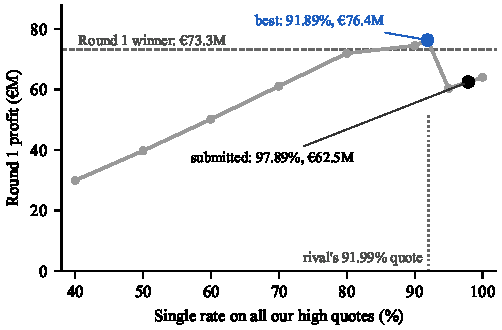
\includegraphics[width=\columnwidth]{fig_replay.pdf}
\caption{Round~1 replayed with all our high quotes set to a single rate, every other offer unchanged.}
\label{fig:replay}
\end{figure}

Table~\ref{tab:r1} shows that the 97.89\% quotes generated 88\% of our profit on a quarter of our loans, and 9{,}230 of those 9{,}239 loans went to applicants whom both rivals refused. Where we competed on price, the winner's curse was real and our correction close: in the 2--4\% band of $p_0$, loans we won defaulted at 3.9\%, loans we lost at 2.5\%, and the model predicted 3.5\% conditional on winning.

What we got wrong was the competitors. Our prior predicted \euro8.6M on 20{,}600 loans; we earned \euro62.5M on 38{,}400. Each rival made offers to only 62--66\% of applicants. It refused about a quarter of even the safest applicants, at the same rate across income, sex and marital status, and at least half of those with $p_0>20\%$. Moreover, one Lender~1 quoted 91.99\% to 14\% of all applicants; it met our 97.89\% quote 9{,}744 times and won every time. Figure~\ref{fig:replay} replays Round~1 with all our high quotes set to one rate: at 91.89\% we would have earned \euro76.4M, more than the winner, while below 80\% the extra loans no longer compensate for the lower margin. Profit came from pricing the applicants that rivals refused, and the level of our high quote mattered far more than the precision of $p_0$.

\section{Round 2 strategy}\label{sec:s2}
\subsection{Learning the rivals' behaviour}
We keep $p_0$ and replace the prior over competitors by their observed behaviour. For a Round~2 applicant $i$, let $N_K(i)$ be the $K=500$ Round~1 applicants with the same employment status and the closest public score $A(x)$. Their rival offers $(r_{1j},r_{3j})$ are draws from what $i$'s rivals will offer, since rivals price on public information and on signals that are independent of ours. An offer also reveals part of the rival's signal, so we re-estimate the default probability on the 100{,}000 Round~1 outcomes:
\begin{multline}\label{eq:wc}
\logit P(D=1\mid p_0,r_1,r_3)=f(\ell)\\
+\sum_{k\in\{1,3\}}\big[g_k(s_k)+\ell\,g'_k(s_k)\big],
\end{multline}
where $\ell=\logit p_0$, $s_k$ is the rank of rival $k$'s offer among offers to applicants with a similar $A(x)$, a refusal is a separate category, and $f$, $g_k$, $g'_k$ are splines. In two-fold cross-fitting, \eqref{eq:wc} lowers the log-loss from 0.2926 for $p_0$ alone to 0.2902. With $\hat p_{ij}=P(D=1\mid p_{0i},r_{1j},r_{3j})$, the expected profit of rate $r$ becomes
\begin{multline}\label{eq:pi2}
\Pi_i(r)=\frac{1}{3K}\sum_{j\in N_K(i)}\sum_{t=1}^{3}\mathbf 1\{r<T_t(r_{1j},r_{3j})\}\\
\times\big[r-(1+r)\,\hat p_{ij}\big],
\end{multline}
which we maximise on a grid of rates ending in 9, up to 99.99\%. In the uniform-adaptation variant of Table~\ref{tab:bt}, larger neighbourhoods (1{,}000 or 2{,}000 applicants), employment effects in \eqref{eq:wc} and a larger safety margin changed backtest profits by at most \euro2.4M, so we kept this specification.

\subsection{Predicting the rivals' reaction}\label{sec:ch}
Best-responding to Round~1 as it was would quote 89.89\%, just under the 91.99\% rival, or 99.99\% to every applicant. Any rival that studies its own diagnostic file can reach the same conclusion, so we model reactions with a cognitive hierarchy \cite{chc2004}. A level-0 rival repeats its Round~1 behaviour. A level-$k$ rival keeps its Round~1 offers below 50\%, but wherever it refused or quoted above 50\% it now quotes
\begin{equation}\label{eq:qk}
q_k(j)=\argmax_{r\ge 0.5}\ \Pi^{(k)}_j(r),
\end{equation}
its profit \eqref{eq:pi2} in a market where each such response is replaced by $q_m$, $m<k$, with probability $f_m/\sum_{l<k}f_l$. Level shares follow $f_k=e^{-\tau}\tau^k/k!$ with the standard $\tau=1.5$, giving 22\%, 34\%, 25\% and 19\% for levels 0, 1, 2 and 3 or more. We approximate the rivals' computation by ours, with the same data.

The hierarchy predicts a ladder of undercutting. The median quote is 89.89\% at level~1, 87.79\% at level~2 and 85.69\% at level~3, while safe applicants, whom many rivals refuse, receive higher quotes (90th percentiles of 99.99\%, 97.89\% and 95.79\%). Our Round~2 rule maximises \eqref{eq:pi2} against this predicted market, in which each high response is replaced by $q_k$ with probability $f_k$.

\begin{table*}[t]
\centering\small
\caption{Cross-fitted backtest on Round~1, profit in \euro M. Each half of the applicants is priced with data from the other half only, then replayed against the actual or perturbed rival offers. Level-$k$: the prediction of Section~\ref{sec:ch}. Wide and narrow: with the stated probability, a rival's refusal or quote above 50\% becomes a uniform draw on [50\%, 95\%] or [85\%, 97\%]. Refusals end: with probability 50\%, a refusal becomes an offer at break-even plus 3 points.}
\label{tab:bt}
\setlength{\tabcolsep}{5pt}
\begin{tabular}{lrrrrrrr}
\toprule
Pricing rule & Unchanged & Level-$k$ & Wide 25\% & Wide 50\% & Narrow 50\% & Refusals end & Mean\\
\midrule
Stage~1 rule (Round~1 file) & 62.5 & 10.6 & 38.5 & 21.5 & 22.7 & 19.5 & 29.2\\
Best response, uniform 25\% adaptation & 121.8 & 72.7 & 77.9 & 44.3 & 98.9 & 40.1 & 76.0\\
Best response to level-$k$ rivals (Round~2 file) & 118.4 & 124.2 & 77.3 & 45.4 & 112.0 & 38.9 & 86.0\\
\bottomrule
\end{tabular}
\end{table*}

\subsection{Backtest and submitted offers}
We cannot observe Round~2 in advance, so we test rules on Round~1 with two-fold cross-fitting and replay them under six rival scenarios (Table~\ref{tab:bt}). The submitted rule earns at least 1.9 times the Stage~1 rule in every scenario. Compared with a rule that simply assumes 25\% of high responses turn into uniform undercuts, it gives up \euro3.4M if rivals do not change, gains \euro51.5M if they react as predicted and has the highest mean.

Our Round~2 file offers a loan to all 100{,}000 applicants: 93.69\% to safe applicants, mostly those with $p_0$ below 4\% (26\% of applicants), and 83.59\% to almost all others (74\%). Both sit just below the predicted level-3 quotes net of the 2-point preference (95.79\% and 85.69\%), so we win even the borrowers who prefer that rival. We thereby stop competing on price: our offers below 20\% earned only \euro7.5M on 28{,}800 loans in Round~1, while about 6\% of safe applicants received no other offer. The model expects \euro123M of profit if rivals react as predicted.

\section{Conclusion}
Round~1 rewarded strategy more than statistics. Our default model was accurate, and most of our profit came from borrowers that rivals refused. In Round~2 we keep the default model, learn the rivals' behaviour from the data and anticipate their reaction with a level-$k$ model. The main risk is a market in which rivals stop refusing altogether; even then, our backtest puts the new rule well ahead of the Stage~1 rule. Our approach has three limitations. First, we assume that rivals reason with our data and our methods, whereas each sees its own signal and its own diagnostic file. Second, the level shares come from laboratory games rather than from this market. Third, almost all our offers sit at two rates, so a rival quoting just below 83.59\% would take most of the borrowers we target; the wide-undercutting scenarios of Table~\ref{tab:bt}, where profit falls to about \euro45M, show the cost of that risk. All results can be reproduced with the scripts and data in our repository, \url{https://github.com/leottawa/Lending-Game}.

\begin{thebibliography}{1}\small
\bibitem{chc2004} C.~F. Camerer, T.-H. Ho and J.-K. Chong (2004). A cognitive hierarchy model of games. \emph{Quarterly Journal of Economics}, 119(3), 861--898.
\end{thebibliography}

\end{document}
